\documentclass{standalone}
\usepackage{tikz}
\usetikzlibrary{patterns, positioning}


\begin{document}
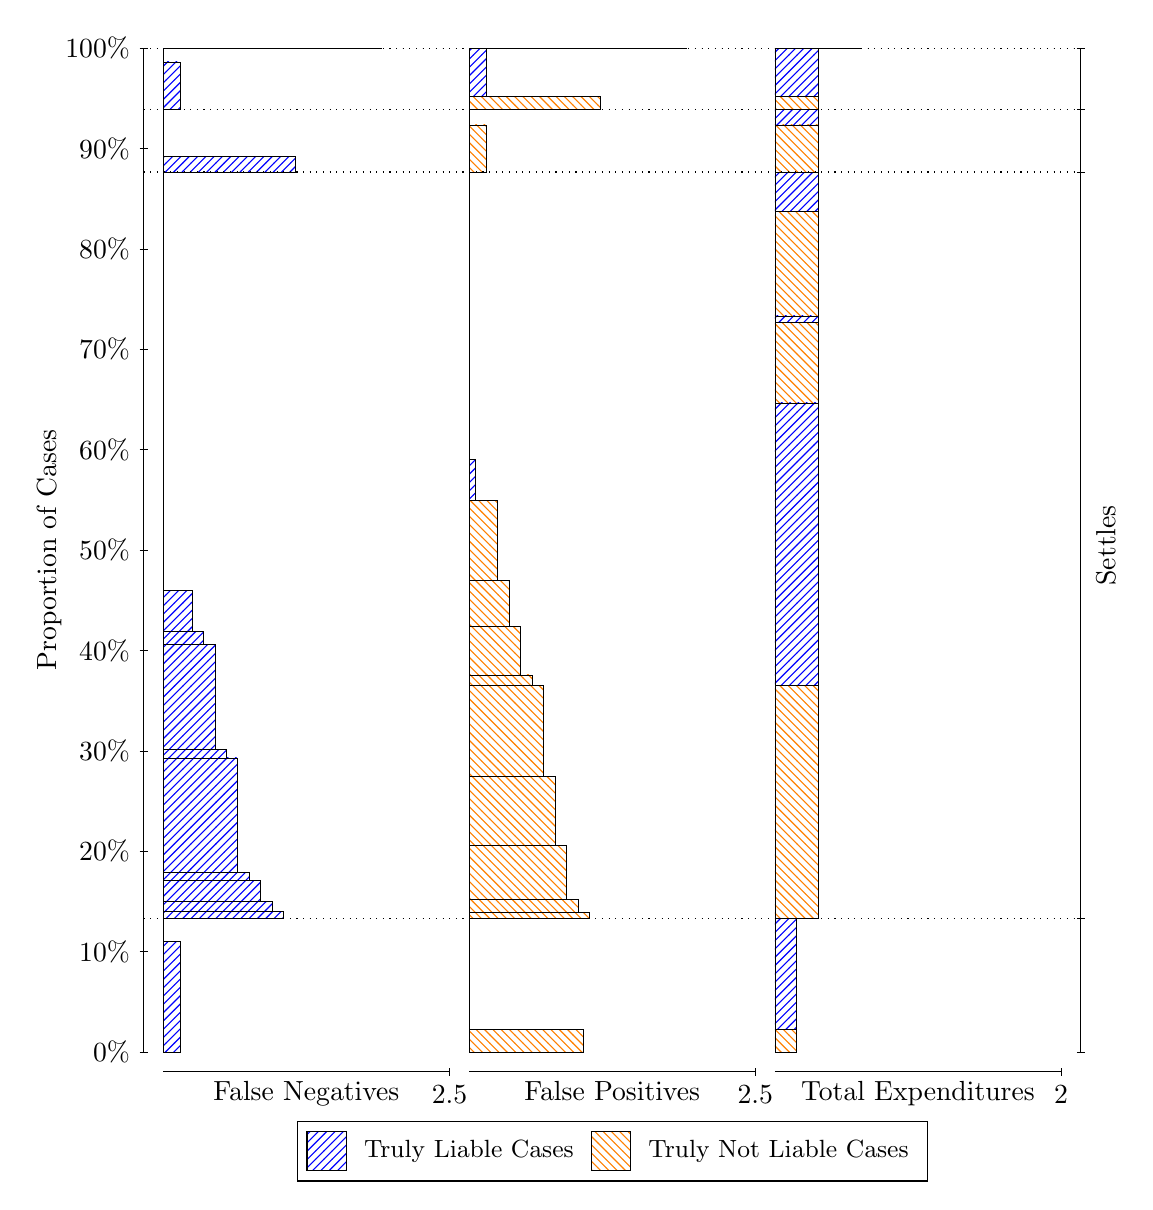
\begin{tikzpicture}
\draw[black, very thin] (1.5,1.75) -- (1.5,14.5);
\node[rotate=90, text=black, anchor=center] at (0.3, 8.125) {Proportion of Cases};
\draw[black, very thin] (1.45,1.75) -- (1.55,1.75);
\node[text=black, anchor=east] at (1.45, 1.75) {0\%};
\draw[black, very thin] (1.45,3.025) -- (1.55,3.025);
\node[text=black, anchor=east] at (1.45, 3.025) {10\%};
\draw[black, very thin] (1.45,4.3) -- (1.55,4.3);
\node[text=black, anchor=east] at (1.45, 4.3) {20\%};
\draw[black, very thin] (1.45,5.575) -- (1.55,5.575);
\node[text=black, anchor=east] at (1.45, 5.575) {30\%};
\draw[black, very thin] (1.45,6.85) -- (1.55,6.85);
\node[text=black, anchor=east] at (1.45, 6.85) {40\%};
\draw[black, very thin] (1.45,8.125) -- (1.55,8.125);
\node[text=black, anchor=east] at (1.45, 8.125) {50\%};
\draw[black, very thin] (1.45,9.4) -- (1.55,9.4);
\node[text=black, anchor=east] at (1.45, 9.4) {60\%};
\draw[black, very thin] (1.45,10.675) -- (1.55,10.675);
\node[text=black, anchor=east] at (1.45, 10.675) {70\%};
\draw[black, very thin] (1.45,11.95) -- (1.55,11.95);
\node[text=black, anchor=east] at (1.45, 11.95) {80\%};
\draw[black, very thin] (1.45,13.225) -- (1.55,13.225);
\node[text=black, anchor=east] at (1.45, 13.225) {90\%};
\draw[black, very thin] (1.45,14.5) -- (1.55,14.5);
\node[text=black, anchor=east] at (1.45, 14.5) {100\%};

\draw[black, very thin] (13.4,1.75) -- (13.4,14.5);
\draw[black, very thin] (13.35,1.75) -- (13.45,1.75);
\node[anchor=west] at (13.35, 1.75) {};
\draw[black, very thin] (13.35,3.4434) -- (13.45,3.4434);
\node[anchor=west] at (13.35, 3.4434) {};
\draw[black, very thin] (13.35,12.925) -- (13.45,12.925);
\node[anchor=west] at (13.35, 12.925) {};
\draw[black, very thin] (13.35,13.719) -- (13.45,13.719);
\node[anchor=west] at (13.35, 13.719) {};
\draw[black, very thin] (13.35,14.492) -- (13.45,14.492);
\node[anchor=west] at (13.35, 14.492) {};
\draw[black, very thin] (13.35,14.496) -- (13.45,14.496);
\node[anchor=west] at (13.35, 14.496) {};
\draw[black, very thin] (13.35,14.5) -- (13.45,14.5);
\node[anchor=west] at (13.35, 14.5) {};

\draw[black, very thin, pattern color=blue, pattern=north east lines] (1.75,1.75) rectangle (1.968,3.1519);
\draw[black, very thin, pattern color=orange, pattern=north west lines] (1.75,3.1519) rectangle (1.75,3.4434);
\draw[black, very thin, pattern color=blue, pattern=north east lines] (1.75,3.4434) rectangle (3.276,3.5322);
\draw[black, very thin, pattern color=blue, pattern=north east lines] (1.75,3.5322) rectangle (3.1307,3.6587);
\draw[black, very thin, pattern color=blue, pattern=north east lines] (1.75,3.6587) rectangle (2.9853,3.9293);
\draw[black, very thin, pattern color=blue, pattern=north east lines] (1.75,3.9293) rectangle (2.84,4.0277);
\draw[black, very thin, pattern color=blue, pattern=north east lines] (1.75,4.0277) rectangle (2.6947,5.4837);
\draw[black, very thin, pattern color=blue, pattern=north east lines] (1.75,5.4837) rectangle (2.5493,5.5883);
\draw[black, very thin, pattern color=blue, pattern=north east lines] (1.75,5.5883) rectangle (2.404,6.9224);
\draw[black, very thin, pattern color=blue, pattern=north east lines] (1.75,6.9224) rectangle (2.2587,7.0963);
\draw[black, very thin, pattern color=blue, pattern=north east lines] (1.75,7.0963) rectangle (2.1133,7.6132);
\draw[black, very thin, pattern color=orange, pattern=north west lines] (1.75,7.6132) rectangle (1.75,12.925);
\draw[black, very thin, pattern color=blue, pattern=north east lines] (1.75,12.925) rectangle (3.4213,13.12);
\draw[black, very thin, pattern color=orange, pattern=north west lines] (1.75,13.12) rectangle (1.75,13.719);
\draw[black, very thin, pattern color=blue, pattern=north east lines] (1.75,13.719) rectangle (1.968,14.323);
\draw[black, very thin, pattern color=orange, pattern=north west lines] (1.75,14.323) rectangle (1.75,14.492);
\draw[black, very thin, pattern color=blue, pattern=north east lines] (1.75,14.492) rectangle (4.5113,14.493);
\draw[black, very thin, pattern color=orange, pattern=north west lines] (1.75,14.493) rectangle (1.75,14.496);
\draw[black, very thin, pattern color=orange, pattern=north west lines] (1.75,14.496) rectangle (1.75,14.497);
\draw[black, very thin, pattern color=blue, pattern=north east lines] (1.75,14.497) rectangle (1.75,14.5);
\draw[black, very thin, pattern color=orange, pattern=north west lines] (5.6333,1.75) rectangle (7.0867,2.0415);
\draw[black, very thin, pattern color=blue, pattern=north east lines] (5.6333,2.0415) rectangle (5.6333,3.4434);
\draw[black, very thin, pattern color=orange, pattern=north west lines] (5.6333,3.4434) rectangle (7.1593,3.5267);
\draw[black, very thin, pattern color=orange, pattern=north west lines] (5.6333,3.5267) rectangle (7.014,3.6897);
\draw[black, very thin, pattern color=orange, pattern=north west lines] (5.6333,3.6897) rectangle (6.8687,4.37);
\draw[black, very thin, pattern color=orange, pattern=north west lines] (5.6333,4.37) rectangle (6.7233,5.2463);
\draw[black, very thin, pattern color=orange, pattern=north west lines] (5.6333,5.2463) rectangle (6.578,6.4071);
\draw[black, very thin, pattern color=orange, pattern=north west lines] (5.6333,6.4071) rectangle (6.4327,6.5403);
\draw[black, very thin, pattern color=orange, pattern=north west lines] (5.6333,6.5403) rectangle (6.2873,7.1567);
\draw[black, very thin, pattern color=orange, pattern=north west lines] (5.6333,7.1567) rectangle (6.142,7.7367);
\draw[black, very thin, pattern color=orange, pattern=north west lines] (5.6333,7.7367) rectangle (5.9967,8.7548);
\draw[black, very thin, pattern color=blue, pattern=north east lines] (5.6333,8.7548) rectangle (5.706,9.2717);
\draw[black, very thin, pattern color=blue, pattern=north east lines] (5.6333,9.2717) rectangle (5.6333,12.925);
\draw[black, very thin, pattern color=orange, pattern=north west lines] (5.6333,12.925) rectangle (5.8513,13.524);
\draw[black, very thin, pattern color=blue, pattern=north east lines] (5.6333,13.524) rectangle (5.6333,13.719);
\draw[black, very thin, pattern color=orange, pattern=north west lines] (5.6333,13.719) rectangle (7.3047,13.888);
\draw[black, very thin, pattern color=blue, pattern=north east lines] (5.6333,13.888) rectangle (5.8513,14.492);
\draw[black, very thin, pattern color=orange, pattern=north west lines] (5.6333,14.492) rectangle (5.6333,14.494);
\draw[black, very thin, pattern color=blue, pattern=north east lines] (5.6333,14.494) rectangle (5.6333,14.496);
\draw[black, very thin, pattern color=orange, pattern=north west lines] (5.6333,14.496) rectangle (8.3947,14.497);
\draw[black, very thin, pattern color=blue, pattern=north east lines] (5.6333,14.497) rectangle (6.9413,14.5);
\draw[black, very thin, pattern color=orange, pattern=north west lines] (9.5167,1.75) rectangle (9.7892,2.0415);
\draw[black, very thin, pattern color=blue, pattern=north east lines] (9.5167,2.0415) rectangle (9.7892,3.4434);
\draw[black, very thin, pattern color=orange, pattern=north west lines] (9.5167,3.4434) rectangle (10.062,6.4071);
\draw[black, very thin, pattern color=blue, pattern=north east lines] (9.5167,6.4071) rectangle (10.062,9.9925);
\draw[black, very thin, pattern color=orange, pattern=north west lines] (9.5167,9.9925) rectangle (10.062,11.011);
\draw[black, very thin, pattern color=blue, pattern=north east lines] (9.5167,11.011) rectangle (10.062,11.099);
\draw[black, very thin, pattern color=orange, pattern=north west lines] (9.5167,11.099) rectangle (10.062,12.429);
\draw[black, very thin, pattern color=blue, pattern=north east lines] (9.5167,12.429) rectangle (10.062,12.925);
\draw[black, very thin, pattern color=orange, pattern=north west lines] (9.5167,12.925) rectangle (10.062,13.524);
\draw[black, very thin, pattern color=blue, pattern=north east lines] (9.5167,13.524) rectangle (10.062,13.719);
\draw[black, very thin, pattern color=orange, pattern=north west lines] (9.5167,13.719) rectangle (10.062,13.888);
\draw[black, very thin, pattern color=blue, pattern=north east lines] (9.5167,13.888) rectangle (10.062,14.492);
\draw[black, very thin, pattern color=orange, pattern=north west lines] (9.5167,14.492) rectangle (10.607,14.494);
\draw[black, very thin, pattern color=blue, pattern=north east lines] (9.5167,14.494) rectangle (10.607,14.496);
\draw[black, very thin, pattern color=orange, pattern=north west lines] (9.5167,14.496) rectangle (10.607,14.497);
\draw[black, very thin, pattern color=blue, pattern=north east lines] (9.5167,14.497) rectangle (10.607,14.5);
\draw[black, dotted] (1.5,3.4434) -- (13.4,3.4434);
\draw[black, dotted] (1.5,12.925) -- (13.4,12.925);
\draw[black, dotted] (1.5,13.719) -- (13.4,13.719);
\draw[black, dotted] (1.5,14.492) -- (13.4,14.492);
\draw[black, dotted] (1.5,14.496) -- (13.4,14.496);
\draw[black, very thin] (1.75,1.5) -- (5.3833,1.5);
\node[text=black, anchor=north] at (3.5667, 1.5) {False Negatives};
\draw[black, very thin] (5.3833,1.45) -- (5.3833,1.55);
\node[text=black, anchor=north] at (5.3833, 1.45) {2.5};

\draw[black, very thin] (5.6333,1.5) -- (9.2667,1.5);
\node[text=black, anchor=north] at (7.45, 1.5) {False Positives};
\draw[black, very thin] (9.2667,1.45) -- (9.2667,1.55);
\node[text=black, anchor=north] at (9.2667, 1.45) {2.5};

\draw[black, very thin] (9.5167,1.5) -- (13.15,1.5);
\node[text=black, anchor=north] at (11.333, 1.5) {Total Expenditures};
\draw[black, very thin] (13.15,1.45) -- (13.15,1.55);
\node[text=black, anchor=north] at (13.15, 1.45) {2};


\node[text=black, centered, rotate=90] at (13.72, 8.184) {Settles};





\draw (7.449999999999999,1.5) node[draw=none] (baseCoordinate) {};
\begin{scope}[align=center]
        \matrix[scale=0.5, draw=black, below=0.5cm of baseCoordinate, nodes={draw}, column sep=0.1cm]{
            \node[rectangle, draw, minimum width=0.5cm, minimum height=0.5cm, pattern color=blue, pattern=north east lines] {}; &
            \node[draw=none, font=\small, text=black] (B) {Truly Liable Cases}; &
            \node[rectangle, draw, minimum width=0.5cm, minimum height=0.5cm, pattern color=orange, pattern=north west lines] {}; &
            \node[draw=none, font=\small, text=black] (B) {Truly Not Liable Cases}; \\
            };
\end{scope}

\end{tikzpicture}
\end{document}